\documentclass[12pt]{article}
\usepackage[left=1cm, right=1cm, top=2cm,bottom=1.5cm]{geometry} 

\usepackage[parfill]{parskip}
\usepackage[utf8]{inputenc}
\usepackage[T2A]{fontenc}
\usepackage[russian]{babel}
\usepackage{enumitem}
\usepackage[normalem]{ulem}
\usepackage{amsfonts, amsmath, amsthm, amssymb, mathtools}

\usepackage{tabularx}
\usepackage{hhline}

\usepackage{accents}
\usepackage{fancyhdr}
\pagestyle{fancy}
\renewcommand{\headrulewidth}{1.5pt}
\renewcommand{\footrulewidth}{1pt}

\usepackage{graphicx}
\usepackage[figurename=Рис.]{caption}
\usepackage{subcaption}
\usepackage{float}

%%Наименование папки откуда забирать изображения
\graphicspath{ {./images/} }

%%Изменение формата для ввода доказательства
\renewcommand{\proofname}{$\square$  \nopunct}
\renewcommand\qedsymbol{$\blacksquare$}

%%Изменение отступа на таблицах
\addto\captionsrussian{%
	\renewcommand{\proofname}{$\square$ \nopunct}%
}
%% Римские цифры
\newcommand{\RN}[1]{%
	\textup{\uppercase\expandafter{\romannumeral#1}}%
}

%% Для удобства записи
\newcommand{\MR}{\mathbb{R}}
\newcommand{\MC}{\mathbb{C}}
\newcommand{\MQ}{\mathbb{Q}}
\newcommand{\MN}{\mathbb{N}}
\newcommand{\MZ}{\mathbb{Z}}
\newcommand{\MTB}{\mathbb{T}}
\newcommand{\MTI}{\mathbb{I}}
\newcommand{\MI}{\mathrm{I}}
\newcommand{\MCI}{\mathcal{I}}
\newcommand{\MJ}{\mathrm{J}}
\newcommand{\MH}{\mathrm{H}}
\newcommand{\MT}{\mathrm{T}}
\newcommand{\MU}{\mathcal{U}}
\newcommand{\MV}{\mathcal{V}}
\newcommand{\MB}{\mathcal{B}}
\newcommand{\MF}{\mathcal{F}}
\newcommand{\MW}{\mathcal{W}}
\newcommand{\ML}{\mathcal{L}}
\newcommand{\MP}{\mathcal{P}}
\newcommand{\VN}{\varnothing}
\newcommand{\VE}{\varepsilon}

\theoremstyle{definition}
\newtheorem{defn}{Опр:}
\newtheorem{rem}{Rm:}
\newtheorem{prop}{Утв.}
\newtheorem{exrc}{Упр.}
\newtheorem{lemma}{Лемма}
\newtheorem{theorem}{Теорема}
\newtheorem{corollary}{Следствие}

\newenvironment{cusdefn}[1]
{\renewcommand\thedefn{#1}\defn}
{\enddefn}

\DeclareRobustCommand{\divby}{%
	\mathrel{\text{\vbox{\baselineskip.65ex\lineskiplimit0pt\hbox{.}\hbox{.}\hbox{.}}}}%
}
%Короткий минус
\DeclareMathSymbol{\SMN}{\mathbin}{AMSa}{"39}
%Длинная шапка
\newcommand{\overbar}[1]{\mkern 1.5mu\overline{\mkern-1.5mu#1\mkern-1.5mu}\mkern 1.5mu}
%Функция знака
\DeclareMathOperator{\sgn}{sgn}

%Функция ранга
\DeclareMathOperator{\rk}{\text{rk}}

%Обозначение константы
\DeclareMathOperator{\const}{\text{const}}

\DeclareMathOperator{\codim}{\text{codim}}

\DeclareMathOperator*{\dsum}{\displaystyle\sum}
\newcommand{\ddsum}[2]{\displaystyle\sum\limits_{#1}^{#2}}

%Интеграл в большом формате
\DeclareMathOperator{\dint}{\displaystyle\int}
\newcommand{\ddint}[2]{\displaystyle\int\limits_{#1}^{#2}}
\newcommand{\ssum}[1]{\displaystyle \sum\limits_{n=1}^{\infty}{#1}_n}

\newcommand{\smallerrel}[1]{\mathrel{\mathpalette\smallerrelaux{#1}}}
\newcommand{\smallerrelaux}[2]{\raisebox{.1ex}{\scalebox{.75}{$#1#2$}}}

\newcommand{\smallin}{\smallerrel{\in}}
\newcommand{\smallnotin}{\smallerrel{\notin}}

\newcommand*{\medcap}{\mathbin{\scalebox{1.25}{\ensuremath{\cap}}}}%
\newcommand*{\medcup}{\mathbin{\scalebox{1.25}{\ensuremath{\cup}}}}%

\makeatletter
\newcommand{\vast}{\bBigg@{3.5}}
\newcommand{\Vast}{\bBigg@{5}}
\makeatother

%Промежуточное значение для sup\inf, поскольку они имеют разную высоту
\newcommand{\newsup}{\mathop{\smash{\mathrm{sup}}}}
\newcommand{\newinf}{\mathop{\mathrm{inf}\vphantom{\mathrm{sup}}}}

%Скалярное произведение
\newcommand{\inner}[2]{\left\langle #1, #2 \right\rangle }
\newcommand{\linsp}[1]{\left\langle #1 \right\rangle }

%Подпись символов снизу
\newcommand{\ubar}[1]{\underaccent{\bar}{#1}}

%% Шапка для букв сверху
\newcommand{\wte}[1]{\widetilde{#1}}
\newcommand{\wht}[1]{\widehat{#1}}

%%Трансформация Фурье
\newcommand{\fourt}[1]{\mathcal{F}\left(#1\right)}
\newcommand{\ifourt}[1]{\mathcal{F}^{-1}\left(#1\right)}

%%Символ вектора
\newcommand{\vecm}[1]{\overrightarrow{#1\,}}

%%Пространстов матриц
\newcommand{\mat}[2]{\operatorname{Mat}_{#1\times #2}}


%%Взятие в скобки, модули и норму
\newcommand{\parfit}[1]{\left( #1 \right)}
\newcommand{\modfit}[1]{\left| #1 \right|}
\newcommand{\sqparfit}[1]{\left\{ #1 \right\}}
\newcommand{\normfit}[1]{\left\| #1 \right\|}

%%Функция для обозначения равномерной сходимости по множеству
\newcommand{\uconv}[1]{\overset{#1}{\rightrightarrows}}
\newcommand{\uconvm}[2]{\overset{#1}{\underset{#2}{\rightrightarrows}}}


%%Функция для обозначения нижнего и верхнего интегралов
\def\upint{\mathchoice%
	{\mkern13mu\overline{\vphantom{\intop}\mkern7mu}\mkern-20mu}%
	{\mkern7mu\overline{\vphantom{\intop}\mkern7mu}\mkern-14mu}%
	{\mkern7mu\overline{\vphantom{\intop}\mkern7mu}\mkern-14mu}%
	{\mkern7mu\overline{\vphantom{\intop}\mkern7mu}\mkern-14mu}%
	\int}
\def\lowint{\mkern3mu\underline{\vphantom{\intop}\mkern7mu}\mkern-10mu\int}


\begin{document}
\lhead{Линейная алгебра и геометрия}
\chead{Тимашев Д.А.}
\rhead{Лекция - 3}
\section*{Фактор-пространства}
Пусть $V$ - фиксированное векторное пространство над полем $K$, $U \subseteq V$ - подпространство в пространстве $V$. Введем на $V$ отношение смежности векторов относительно подпространства.

\begin{defn}
	Говорят, что вектор $v$ \uwave{смежен} вектору $v'$ относительно подпространства $U$, если:
	$$
		\exists \, u \in U \colon v = v' + u
	$$
	И записывать будем это следующим образом: $v \underset{U}{\sim} v'$. Когда $U$ фиксировано, будем просто писать: $v \sim v'$.
\end{defn}

\begin{prop}
	Смежность это отношение эквивалентности.
\end{prop}
\begin{proof}\hfill
	\begin{enumerate}[label=\arabic*)]
		\item \textbf{Рефлексивность}: $v \sim v$
		$$
			0 \in U, \, v + 0 = v \Rightarrow v \sim v
		$$
		\item \textbf{Симметричность}: $v \sim v' \Rightarrow  v' \sim v$
		$$
			v \sim v' \Rightarrow v = v' + u, \, u \in U \Rightarrow  v' = v + (-u), \, -u \in U \Rightarrow v' \sim v
		$$
		\item \textbf{Транзитивность}: $v \sim v', \, v' \sim v'' \Rightarrow v \sim v''$
		$$
			v \sim v', \, v' \sim v'' \Rightarrow  v = v' + u,\, v' =v'' + u', \, u,u' \in U \Rightarrow v = v'' + (u + u'), \, u + u' \in U \Rightarrow v \sim v''
		$$
	\end{enumerate}
\end{proof}
Как мы знаем, отношение эквивалентности на множестве разбивает множество на попарно непересекающиеся классы эквивалентности. Внутри одного класса все элементы эквивалентны.
\begin{defn}
	Классы эквивалентности по смежности относительно подпространства $U$ называются \uwave{смежными классами} по подпространству $U$. Смежный класс вектора $v \in V$ - это множество: 
	$$
		v +U = \{v' \in V \mid v' \sim v \} = \{v' \in V \mid v'= v + u, \, u \in U \}
	$$
\end{defn}

\begin{defn}
	\uwave{Фактор-пространство} $V /U$ векторного пространства $V$ по подпространству $U$, это множество всех смежных классов в пространстве $V$ по $U$ на котором задана структура векторного пространства с помощью операций:
	\begin{enumerate}
		\item[($+$):] $\forall v,w \in V, \, (v + U) + (w + U) = v + w + U$;
		\item[($\; \cdot \; $):] $\forall v \in V, \, \forall \lambda \in K, \, \lambda{\cdot}(v + U) = \lambda{\cdot}v + U$;
	\end{enumerate}
\end{defn}
Необходимо проверить, что операции над смежными классами определены корректно, то есть результат не зависит от того, каких представителей мы выберем в данных двух смежных классах.

Аксиомы векторного пространства для $V/U$ вытекают из аксиом векторного пространства для $V$, поскольку операции над смежными классами определяются с помощью операций над представителями этих смежных классов, т.е. над самими векторами из пространства $V$.

\begin{rem}
	Нулевой вектор в $V/U$: $0 + U = U$.
\end{rem}

\newpage
\begin{prop}(\textbf{Корректность определения})
	Определение фактор-пространства не зависит от выбора представителей смежных классов.
\end{prop}
\begin{proof}
	Пусть $v' \sim v, \, w' \sim w$, тогда:
	$$
		v' \sim v, \, w' \sim w \Rightarrow v' = v + u, \, w' = w + u', \, u,u' \in U \Rightarrow v' + w' = v + w + \underbrace{u + u'}_{\in U} \Rightarrow v' + w' \sim v + w
	$$
	То есть, если выбрать вместо $v$ и $w$ два других представителя тех же самых смежных классов, то результат попадет в тот же смежный класс, что и в определении $\Rightarrow$ операция суммы не зависит от выбора представителя. Аналогичное мы получим и для умножения на скаляр:
	$$
		\lambda{\cdot}v' = \lambda {\cdot}v + \lambda{\cdot}u, \, \lambda{\cdot}u \in U \Rightarrow \lambda{\cdot}v' \sim \lambda{\cdot}v
	$$
\end{proof}

\subsection*{Примеры фактор-пространств}

$1)$ $V = \{\text{геом. векторы в пространстве}\}, \, U = \{\text{геом. векторы в данной фикс. плоскости}\}$.

Выберем начало координат в $V$, будем откладывать все векторы от этой точки $0$. Будем считать $U$ проходящей через эту точку.
\begin{figure}[H]
	\centering
	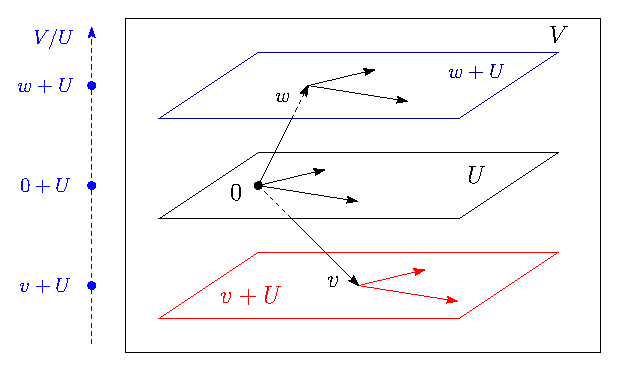
\includegraphics[width=0.65\textwidth]{LAL3_1.eps}
	\caption{Смежные классы у фактор-пространства $V/U$.}
	\label{3_1}
\end{figure}
Если рассматривать всевозможные векторы из начала координат идущие в разные точки пространства,  это и будет нашим векторным пространством $V$. Смежным классом будет прибавление к фиксированному вектору $v$ или $w$ всевозможных векторов пространства $U$. 

Мы получим векторы, концы которых лежат на плоскости параллельной плоскости $U$, но проходящие через конец вектора $v$ или $w$. Фактор-пространство это множество этих смежных классов, то есть множество параллельных плоскостей, на которые расслаивается геометрическое пространство $V$. Можно мысленно его представлять как вертикальную прямую, которая параметризует множество паралелльных плоскостей (точки на прямой задают смежные классы).

\newpage
$2)$ $V = \MF(X,K),\, Y \subseteq X, \, U = \MCI(Y) = \{g \colon X \to K \mid g(y) = 0, \, ,\forall y \in Y\} $, тогда $V/U \simeq \MF(Y,K)$. Построим этот изоморфизм. Утверждается, что: $f + \MCI(Y) \mapsto f|_Y$ - взаимнооднозначное, то есть: 
$$
	f + \MCI(Y) \leftrightarrow f|_Y
$$

\textbf{\uline{Корректность}}: $f \sim f' \Rightarrow f = f' + g, \, g|_Y = 0 \Rightarrow  f|_Y = f'|_Y + g|_Y = f'|_Y$.

\textbf{\uline{Биективность}}: $f|_Y = f'|_Y \Rightarrow g = f - f' \in \MCI(Y) \Rightarrow f \sim f' \Rightarrow$ инъективно. Сюръективность - очевидна, поскольку $\forall f \colon Y \to K$  может быть продолжена до функции на $X$.

\textbf{\uline{Согласованность}}: $f + \MCI(Y) + h + \MCI(Y) \mapsto f|_Y + h|_Y$, $\lambda{\cdot}(f + \MCI(Y)) = \lambda{\cdot}f|_Y + \MCI(Y) \to \lambda{\cdot}f|_Y$. 

\begin{prop}
	Пусть $\dim{V} < \infty$, тогда: 
	$$
		\dim{(V/U)} = \dim{V} - \dim{U}
	$$
\end{prop}
\begin{proof}
	Выберем согласованный базис: $(e_1, \dotsc, e_k, e_{k+1}, \dotsc, e_n)$ - базис $V$ и $(e_{k+1}, \dotsc, e_n)$ - базис $U$.
	\begin{figure}[H]
		\centering
		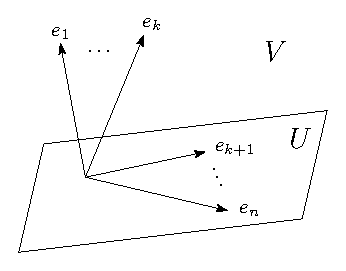
\includegraphics[width=0.25\textwidth]{LAL3_2.eps}
		\caption{Выбор согласованного базиса $V$ с подпространством $U$.}
		\label{3_2}
	\end{figure}
	Докажем, что $(e_1 + U, \dotsc, e_k + U)$ - базис $V/U$. По определению:
	$$
		\forall v \in V, \, \exists \, \lambda_1 ,\dotsc,\lambda_n \in K \colon v = \lambda_1 e_1 + \dotsc + \lambda_k e_k + \lambda_{k+1} e_{k+1} + \dotsc + \lambda_n e_n
	$$
	Заметим, что $\lambda_{k+1} e_{k+1} + \dotsc + \lambda_n e_n \in U$. Отсюда следует, что смежный класс вектора $v$ представляется в виде линейной комбинации смежных классов векторов $e_1, \dotsc, e_k$ с теми же коэффициентами:
	$$
		v + U  = \lambda_1 (e_1 + U) + \dotsc + \lambda_k(e_k + U)
	$$
	Следовательно, $(e_1 + U, \dotsc, e_k + U)$ порождает $V/U$. Докажем линейную независимость. Пусть:
	$$
		\mu_1(e_1 + U) + \dotsc + \mu_k(e_k + U) = U \Rightarrow \mu_1 e_1 + \dotsc + \mu_k e_k \in U \Rightarrow 
	$$
	$$
		 \Rightarrow\mu_1 e_1 + \dotsc + \mu_k e_k = \mu_{k+1}e_k{k+1} + \dotsc + \mu_n e_n \Rightarrow \mu_1 e_1 + \dotsc + \mu_k e_k - \mu_{k+1}e_k{k+1} - \dotsc - \mu_n e_n = 0
	$$
	Но линейная комбинация базисных векторов равна нулю, только если коэффициенты равны нулю: 
	$$
		\mu_1 = \dotsc = \mu_k = \mu_{k+1} = \dotsc = \mu_n = 0
	$$
	Следовательно, $(e_1 + U, \dotsc, e_k + U)$ - базис $V/U$ и мы получаем размерности: 
	$$
		\dim{(V/U)} = k, \, \dim{V} = n, \, \dim{U} = n - k
	$$
\end{proof}

\begin{defn}
	\uwave{Коразмерность подпространства} $U \subseteq V$ это размерность фактор-пространства $V/U$:
	$$
		\codim{U} = \dim{(V/U)}
	$$
\end{defn}
\begin{rem}
	Заметим, что возможен случай бесконечномерного $V$ и его подпространства $U$, но при этом конечномерного фактор-пространства. 
\end{rem}

\textbf{Пример}: $V = \MF(X,K), \, U = \MCI (Y) \simeq \MF(X\setminus Y,K)$, где изоморфность следует из того, что такие функции полностью определяются значениями на дополнении к множеству $Y$.

Также, как и ранее $V/U \simeq \MF(Y,K)$. Если $X$ - бесконечно, а $|Y| = n$, тогда $V$ и $U$ будут бесконечномерными, поскольку пространство функций на бесконечном множестве - бесконечномерное. Функция на конечном множестве определяется просто набором своих значений: если множество из $n$ элементов, то это будет набор из $n$ значений $\Rightarrow V / U \simeq K^n \Rightarrow \dim{(V/U)} = n < \infty$.

\newpage
\section*{Прямая сумма}
Пусть $U_1, \dotsc, U_m \subseteq V$ - подпространства.
\begin{defn}
	Подпространства $U_1, \dotsc, U_m$ называются \uwave{линейно независимыми}, если выполнено:
	$$
		u_1 + \dotsc + u_m = 0, \, u_i \in U_i, \, i =\overline{1,m} \Rightarrow u_1 = \dotsc = u_m = 0
	$$
\end{defn}

\begin{prop}
	Следующие условия эквивалентны:
	\begin{enumerate}[label=(\arabic*)]
		\item $U_1, \dotsc, U_m$ - линейно независимы;
		\item $\forall i = \overline{1,m}, \, U_i \cap \left(U_1 + \dotsc + U_{i-1} + U_{i+1} + \dotsc + U_{m}\right) = \{0\}$;
		\item $\forall v \in U_1 + \dotsc + U_m, \, \exists! \, u_i \in U_i, \, i = \overline{1,m}\colon v = u_1 + \dotsc + u_m$;
	\end{enumerate}
\end{prop}
\begin{proof}\hfill\\
	$(1) \Rightarrow (3)$ Пусть разложение не единственное:
	$$
		v = u_1 + \dotsc + u_m = u'_1 + \dotsc + u'_m, \, (\forall i = \overline{1,m}, \, u_i, u'_i \in U_i)
	$$ 
	тогда вычтем одно из другого и получим:
	$$
		(u_1 - u'_1) + \dotsc + (u_m - u'_m) = 0, \, \forall i = \overline{1,m}, \, u_i - u'_i \in U_i
	$$
	По условию $(1)$ мы получаем, что $\forall i = \overline{1,m}, \, u_i - u'_i = 0 \Rightarrow u_i = u'_i$.
	
	$(3) \Rightarrow (2)$ Пусть $u_i \in  U_i \cap \left(U_1 + \dotsc + U_{i-1} + U_{i+1} + \dotsc + U_{m}\right)$, тогда этот вектор может быть представлен в виде суммы векторов из суммы подпространств (как части пересечения):
	$$
		u_i = u_1 + \dotsc + u_{i-1} + 0 + u_{i+1} + \dotsc + u_m, \, \forall u_j \in U_j
	$$
	Но тот же самый вектор $u_i$ может быть разложен по-другому:
	$$
		u_i = 0 + \dotsc + 0 + u_i + 0 + \dotsc + 0
	$$
	Это то же разложение вектора, а поскольку из $(3)$ разложение единственное, то: 
	$$
		u_1 = \dotsc = u_i = \dotsc = u_m = 0
	$$
	
	$(2) \Rightarrow (1)$ Пусть $u_1 + \dotsc + u_m = 0$, где $u_1 \in U_1, \dotsc, u_m \in U_m$, тогда мы можем перенести слагаемые в правую часть и переписать равенство в следующем виде:
	$$
		\forall i = \overline{1,m}, \, u_i = - u_1 - \dotsc - u_{i-1} - u_{i+1} - u_m \in U_i \cap \left(U_1 + \dotsc + U_{i-1} + U_{i+1} + \dotsc + U_{m}\right) \Rightarrow
	$$
	$$
		\Rightarrow \forall i = \overline{1,m}, \, u_i = 0
	$$
	В силу того, что пункт $(2)$ - верный $\Rightarrow$ условие линейной независимости выполняется.
\end{proof}

\begin{rem}
	В \uline{\textbf{частном случае}}, когда подпространства $U,W \subseteq V$ - линейно независимы $\Leftrightarrow U \cap W = \{0\}$. \\ Также заметим, что когда подпространств больше, чем $2$, то нулевого пересечения недостаточно, чтобы они были линейно независимы, более того, недостаточно даже попарного пересечения любых двух подпространств. Примеры будут на семинаре.
\end{rem}

\begin{defn}
	Сумма $U = U_1 + \dotsc + U_m$ называется \uwave{прямой суммой} (внутренней прямой суммой) подпространств, если $U_1,\dotsc, U_m$ - линейно независимы. \uline{\textbf{Обозначение}}: $U = U_1 \oplus \dotsc \oplus U_m$.
\end{defn}
По утверждению $4$, для любого вектора $v \in U_1 \oplus \dotsc \oplus U_m$ существует его единственное разложение в сумму векторов из слагаемых этой прямой суммы:
$$
	v = u_1 + \dotsc + u_m, \, u_i \in U_i
$$

\begin{defn}
	Слагаемые $u_i, \, i = \overline{1,m}$ в разложении $v \in U_1 \oplus \dotsc \oplus U_m$, называются \uwave{проекциями} вектора $v$ на слагаемые прямой суммы.
\end{defn}

\subsection*{Примеры прямых сумм}

$1)$ Рассмотрим стандартное пространство: $V = \{\text{геом. вектора в пространстве}\}$ и его подпространства: $U = \{\text{геом. векторы на плоскости }P\}$ и $W = \left\{\text{геом. векторы на прямой }l\nparallel P\right\}$, тогда: $V = U \oplus W$.
\begin{figure}[H]
	\centering
	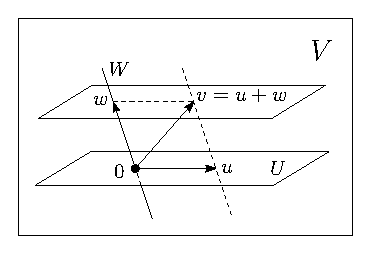
\includegraphics[width=0.3\textwidth]{LAL3_3.eps}
	\caption{Пример прямой суммы геом. пространства.}
	\label{3_3}
\end{figure}
Для удобства берём начало координат и все векторы откладываем от этого начала. Плоскость $U$ будет проходить через эту точку, прямая $W$ будет проходить через начало координат и будет $\parallel l$. Заметим, что их пересечение только в точке $0$. Покажем, что $\forall v \in V$ он единственным способом разлагается в сумму векторов из $U$ и $W$.

Возьмем произвольный $v \in V$, через конец $v$ проведём прямую $\parallel W$ и там, где она пересечет $U$ мы получим $u$ - вектор-проекцию на $U$, аналогично, через конец $v$ проведем плоскость $\parallel U$ и там, где она пересечет $W$ мы получим $w$ - вектор-проекцию на $W \Rightarrow v = u + w$.
\begin{rem}
	Заметим, что проекции не ортогональные, никакой перпендикулярности здесь не требуется.
\end{rem}

$2)$  $\dim{V} = n < \infty, \, (e_1, \dotsc, e_n)$ - базис $V$, тогда $V = U_1 \oplus \dotsc \oplus U_m$, где $\forall i = \overline{1,m}, \, U_i = \linsp{e_i}$. 
\begin{figure}[H]
	\centering
	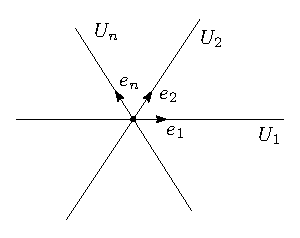
\includegraphics[width=0.24\textwidth]{LAL3_4.eps}
	\caption{Пример прямой суммы конечномерного пространства.}
	\label{3_4}
\end{figure}
Это вытекает из определения базиса, поскольку любой вектор $v \in V$ единственным способом разлагается в виде линейной комбинации базисных векторов, а векторы пропорциональные базисным это как раз векторы из этих одномерных подпространств $\Rightarrow$ эти подпространства линейно независимы и образуют прямую сумму.

$3)$ $\mat{n}{n}{(K)} = \operatorname{Sym}_{n\times n}{(K)} \oplus \operatorname{Skew}_{n\times n}{(K)}$, где $ Sym_{n\times n}{(K)}$ - пространство симметрических матриц размера $n$ на $n$ и $Skew_{n\times n}{(K)}$ - пространство кососимметрических матриц размера $n$ на $n$.  Дополнительно потребуем, чтобы $\operatorname{char}{K} \neq 2$.
\begin{prop}
	$\forall A \in \mat{n}{n}{(K)}, \, \exists! \, B \in  \operatorname{Sym}_{n\times n}{(K)}, \, C \in \operatorname{Skew}_{n\times n}{(K)} \colon A = B + C$.
\end{prop}
\begin{proof}\hfill\\
	\textbf{\uline{Единственность}}: Пусть $A = B + C \Rightarrow A^T = B^T + C^T = B - C \Rightarrow B = \dfrac{A + A^T}{2}, \, C = \dfrac{A - A^T}{2}$. Если бы характеристика поля была бы равна $2$, то мы бы не смогли поделить на двойку, потому что двойка равна нулю $\Rightarrow$ не нашли бы матрицы $B$ и $C$.
	
	\textbf{\uline{Существование}}: Положим, что $B = \dfrac{A + A^T}{2}, \, C = \dfrac{A - A^T}{2}$, тогда легко видеть, что: 
	$$
		B^T = \dfrac{A^T + A}{2} = B, \, C^T = \dfrac{A^T - A}{2} = - C \Rightarrow B \in  \operatorname{Sym}_{n\times n}{(K)}, \, C \in \operatorname{Skew}_{n\times n}{(K)}
	$$
\end{proof}
\section*{Прямая внешняя сумма}

\begin{defn}
	Пусть $V_1, \dotsc, V_m$ - векторные  пространства, их \uwave{внешняя прямая сумма} $V_1 \oplus \dotsc \oplus V_m$ это векторное пространство на множестве упорядоченных наборов векторов (Декартово произведение):
	$$
		V_1 \oplus \dotsc \oplus V_m = \{(v_1, \dotsc, v_m) \mid v_i \in V_i, \, \forall i = \overline{1,m}\}
	$$
	на котором структура векторного пространства задана покомпонентно:
	\begin{enumerate}
		\item[($+$):] 	$\forall v,w \in V_1 \oplus \dotsc \oplus V_m, \, v + w = (v_1 ,\dotsc, v_m)  + (w_1,\dotsc, w_m) = (v_1 + w_1, \dotsc , v_m + w_m)$;
		\item[($\; \cdot \; $):] $\forall v \in V_1 \oplus \dotsc \oplus V_m, \, \forall \lambda \in K, \, \lambda {\cdot}v = \lambda {\cdot} (v_1 ,\dotsc, v_m) = (\lambda v_1, \dotsc, \lambda v_m)$;
	\end{enumerate}
\end{defn}

\textbf{Пример}: $K^n = \underbrace{K \oplus  \dotsc \oplus K}_{n}$.

\begin{rem}
	Внутренняя прямая сумма подпространств $U = U_1 \oplus \dotsc \oplus U_m$ изоморфна внешней прямой сумме этих пространств, потому что каждый вектор из внутренней прямой суммы однозначно разлагается в сумму своих проекций на слагаемые и мы можем сопоставить этому вектору набор этих проекций:
	$$
		\forall v \in U, \, \exists! \, v = u_1 + \dotsc + u_m,\, u_i \in U_i \Rightarrow v \leftrightarrow (u_1,\dotsc, u_m) 
	$$
	где $(u_1,\dotsc, u_m)$ - элемент внешней прямой суммы, по свойству единственности разложения по прямым слагаемым это соответствие будет взаимнооднозначным и изоморфизмом (проверяется покомпонентно). И наоборот, всякая внешняя прямая сумма $V_1 \oplus \dotsc \oplus V_m$ является внутренней. Предъявим разложение:
	$$
		V_1 \oplus \dotsc \oplus V_m = U_1 \oplus \dotsc \oplus U_m, \, U_i = \underset{1}{\{0\}} \oplus \dotsc \oplus \underset{i}{V_i\vphantom{\{0\}}} \oplus \dotsc \oplus \underset{m}{\{0\}}
	$$
	$$
		(v_1,\dotsc,v_m) = \ddsum{i = 1}{m}(\underset{1}{0\vphantom{v_i}}, \dotsc, \underset{i-1}{0\vphantom{v_i}}, \underset{i}{v_i}, \underset{i+1}{0\vphantom{v_i}}, \dotsc, \underset{m}{0\vphantom{v_i}})
	$$
	Легко видеть, что $U_i$ - подпространства во внешней прямой сумме и они удовлетворяют определению внутренней прямой суммы: каждый набор представляется единственным способом в виде суммы наборов выше, где на всех местах нули, кроме одного, то есть - представление в виде суммы выше - единственное.
\end{rem}

\begin{theorem}
	Пусть $\dim{V} < \infty$, $U_1, \dotsc, U_m \subseteq V$  - подпространства, тогда следующие условия эквивалентны:
	\begin{enumerate}[label=(\arabic*)]
		\item $U_1,\dotsc, U_m$ - линейно независимы;
		\item Объединение базисов $U_1, \dotsc, U_m$ есть базис $U_1 + \dotsc + U_m$;
		\item $\dim{(U_1 + \dotsc + U_m)} = \dim{U_1} + \dotsc + \dim{U_m}$;
	\end{enumerate}
\end{theorem}
\begin{proof}
	Без ограничения общности, можно считать, что $U_1 + \dotsc + U_m = V$, если это не так, то уменьшим это пространство до суммы. Выберем в каждом $U_i$ - базис:
	$$
		\forall i = \overline{1,m}, \, e_{i,\cdot} = (e_{i,1}, e_{i,2}, \dotsc, e_{i, n_i}), \, n_i = \dim{U_i} \Rightarrow V = \linsp{e_{ij} \mid i = \overline{1,m},\, j = \overline{1,n_i}}
	$$
	
	$(1) \Rightarrow (2)$ Достаточно доказать линейную независимость $e_{ij} \Rightarrow$ это будет базис. Рассмотрим линейную комбинацию равную нулю и разобъем сумму на группы:
	$$
		\ddsum{\substack{i = 1,\dotsc,m\\j = 1,\dotsc, n_i}}{}\lambda_{ij} e_{ij} = \ddsum{i = 1}{m}\Bigg(\underbrace{\ddsum{j = 1}{n_i}\lambda_{ij}e_{ij}}_{\smallin U_i}\Bigg) = 0 
	$$
	Из линейной независимости $U_i$, каждое слагаемое в сумме должно быть равно нулю:
	$$
		\forall i = \overline{1,m}, \, \ddsum{j = 1}{n_i}\lambda_{ij}e_{ij} = 0 \Rightarrow \forall i = \overline{1,m}, j = \overline{1,n_i}, \, \lambda_{ij} = 0
	$$
	где последнее верно в силу того, что $e_{i,\cdot}$ - базисы у $U_i$.
	
	$(2) \Rightarrow (1)$ Обратно, мы хотим доказать, что подпространства $U_1, \dotsc, U_m$ - линейно независимы. Пусть верно $u_1 + \dotsc + u_m = 0, \, u_i \in U_i$. Разложим каждый из этих векторов:
	$$
		\forall i = \overline{1,m}, \, u_i = \ddsum{j = 1}{n_i}\lambda_{ij}e_{ij}  \Rightarrow u_1 + \dotsc + u_n = \ddsum{\substack{i = 1,\dotsc,m\\j = 1,\dotsc, n_i}}{}\lambda_{ij} e_{ij} = 0 \Rightarrow 
	$$
	$$
		\Rightarrow \forall i = \overline{1,m}, j = \overline{1,n_i}, \, \lambda_{ij} = 0 \Rightarrow u_i = 0, \, \forall i =\overline{1,m}
	$$
	где мы воспользовались тем, что $(e_{11}, \dotsc, e_{mn_m})$ - базис $U$.
	
	$(2) \Rightarrow (3)$ Очевидно, поскольку объединям базисы разных подпространств и получаем базис всего пространства $\Rightarrow$ их количества суммируются $\Rightarrow$ размерность суммы равна сумме разамерностей.
	
	$(3) \Rightarrow (2)$ Мы знаем, что векторы $e_{ij}$ порождают всё $V = U_1 + \dotsc + U_m$, а их количество равно сумме размерностей: $n_1 + \dotsc + n_m = \dim{U_1} + \dotsc + \dim{U_m}$. Если бы эти векторы были линейно зависимы, то их систему можно было бы уменьшить до базиса $\Rightarrow$ в базисе будет меньшее количество векторов, тогда:
	$$
		\dim{V} = \dim{(U_1 + \dotsc +U_m)} < \dim{U_1} + \dotsc + \dim{U_m}
	$$ 
	Получаем противоречие $\Rightarrow$ векторы линейно независимы $\Rightarrow$ образуют базис.
\end{proof}

\end{document}